\documentclass{article}
\usepackage{iclr2026_conference,times}
\input{math_commands.tex}
\usepackage{hyperref}
\usepackage{url}
\usepackage{booktabs}
\usepackage{graphicx}
\usepackage{microtype}

\title{Sensor Failure Compositionality for Multimodal Robot Policies}
\author{Anonymous Authors}

\begin{document}
\raggedbottom
\maketitle

\begin{abstract}
Multimodal robots are usually tested against missing or corrupted sensors one modality at a time. That is a weak deployment model: a blurred camera, drifting force-torque estimate, and delayed tactile recovery can combine into an error that is not predicted by any single-failure diagnostic. We rebuild and re-audit Paper 103 around a falsifiable hypothesis: policies should represent \emph{sensor failure composition}, i.e., higher-order interactions between failed or unreliable modalities that change the recovery action. The resulting local benchmark covers 5 robot task families, 7 sensor-failure families, 5 stress splits, 9 methods, 7 seeds, and 84 episodes per group. On the 2026-06-15 continuation rerun, the proposed compositional model obtains $0.6071 \pm 0.0055$ success versus $0.5441 \pm 0.0064$ for the strongest non-oracle baseline, while lowering safety violation from $0.2345$ to $0.1960$ and damage from $0.1594$ to $0.1342$. Pairwise tests favor the proposed method over the strongest baseline in 7/7 seeds, and ablations show that cross-sensor interaction edges, disagreement features, conformal gating, and recovery-action selection each matter. The terminal decision is \textbf{STRONG\_REVISE}: the local evidence supports the mechanism, but the paper is not ICLR-main-ready until validated on real robots or independent high-fidelity benchmarks.
\end{abstract}

\section{Why this paper exists}
Sensor failures are not rare corner cases. Robot sensors wear, saturate, desynchronize, drift, occlude, and disagree. Prior work already studies sensor dropout for robust policies \citep{liu2017sensor,peri2024masked}, multimodal robot failure detection \citep{inceoglu2024fino}, conformal safety alarms \citep{luo2024conformal}, robust tactile sensing \citep{zhao2025polytouch}, and robust autonomous-driving sensor fusion under adverse failures \citep{park2025mome}. A generic claim of ``more robust multimodal fusion'' would therefore be too crowded.

The narrower claim is that \emph{combinations} of sensor failures can change the diagnosis and the correct recovery action. Independent fault detectors can discover that vision is unreliable and tactile is delayed; they do not necessarily know whether that pair creates a different failure mode than either fault alone. Paper 103 tests whether explicitly modeling those interaction terms improves success, safety, and recovery diagnostics under paired and combined stress.

\section{Method sketch}
The proposed method is a compositional failure graph over seven evidence channels: vision, tactile, proprioception, force-torque, depth, language grounding, and cross-modal disagreement. Nodes estimate marginal reliability. Edges estimate interaction load, such as vision-depth miscalibration during obstacle avoidance or tactile-force disagreement during insertion. The policy monitor scores:
\begin{itemize}
\item marginal single-sensor load,
\item pairwise interaction load,
\item delayed recovery state,
\item false-isolation risk, and
\item recovery-action utility.
\end{itemize}

The benchmark implements this mechanism as an executable diagnostic policy model rather than a trained neural checkpoint. That choice keeps the local evidence reproducible and RAM-light, but it is also the main reason the paper remains strong-revise rather than submission-ready.

\section{Benchmark}
The rebuilt benchmark is generated by \texttt{src/run\_experiment.py}. It stores aggregate CSVs rather than trajectories, so the full run remains lightweight without dropping experimental coverage.

\paragraph{Tasks.}
The tasks are grasp selection, insertion/alignment, deformable handling, mobile manipulation near obstacles, and tool-use contact control.

\paragraph{Failure families.}
The sensor-failure families are vision-only, tactile-only, proprioception-only, force-torque-only, depth-only, language-grounding-only, and compositional multi-sensor interaction.

\paragraph{Splits.}
The stress splits are nominal, single-sensor shift, paired-sensor shift, delayed sensor recovery, and combined stress.

\paragraph{Methods.}
The non-oracle baselines are a nominal multimodal policy, sensor-dropout augmentation, independent fault detectors, ensemble uncertainty gating, conformal sensor-reliability filtering, Bayesian sensor-fusion monitoring, and a robust single-worst-sensor policy. The benchmark also includes the proposed sensor-failure composition model and an oracle failure-aware policy.

\paragraph{Metrics.}
The evidence reports success, safety violation, damage, fault-detection F1, interaction-detection F1, false isolation, recovery latency, total cost, regret to oracle, paired seed differences, ablations, stress sweeps, and failure cases.

\section{Results}
% Auto-generated by src/run_experiment.py
\begin{table}[t]
\centering
\caption{Combined-stress sensor-failure-compositionality benchmark.}
\begin{tabular}{lrrrrrr}
\toprule
Method & Succ. & Viol. & Dmg. & InterF1 & Latency & Regret \\
\midrule
Oracle & 0.737 & 0.152 & 0.100 & 0.676 & 0.511 & 0.000 \\
Proposed & 0.607 & 0.196 & 0.134 & 0.560 & 0.620 & 0.130 \\
BayesFusion & 0.544 & 0.235 & 0.159 & 0.370 & 0.767 & 0.193 \\
EnsUncert & 0.503 & 0.237 & 0.153 & 0.282 & 0.827 & 0.233 \\
WorstSensor & 0.503 & 0.218 & 0.133 & 0.297 & 0.815 & 0.234 \\
IndFault & 0.502 & 0.262 & 0.175 & 0.267 & 0.860 & 0.234 \\
ConfReliab & 0.501 & 0.230 & 0.143 & 0.300 & 0.833 & 0.236 \\
DropoutAug & 0.438 & 0.274 & 0.191 & 0.195 & 0.883 & 0.299 \\
Nominal & 0.377 & 0.283 & 0.196 & 0.143 & 0.924 & 0.360 \\
\bottomrule
\end{tabular}
\end{table}


The strongest non-oracle baseline is \texttt{bayesian\_sensor\_fusion\_monitor}. On combined stress, the proposed model improves success by $0.0631 \pm 0.0088$, wins 7/7 paired seeds, lowers safety violation by $0.0385$, and lowers damage by $0.0253$. The oracle remains substantially better at $0.7368 \pm 0.0070$, which is a useful sanity check: the benchmark is not saturated.

\begin{figure}[t]
\centering
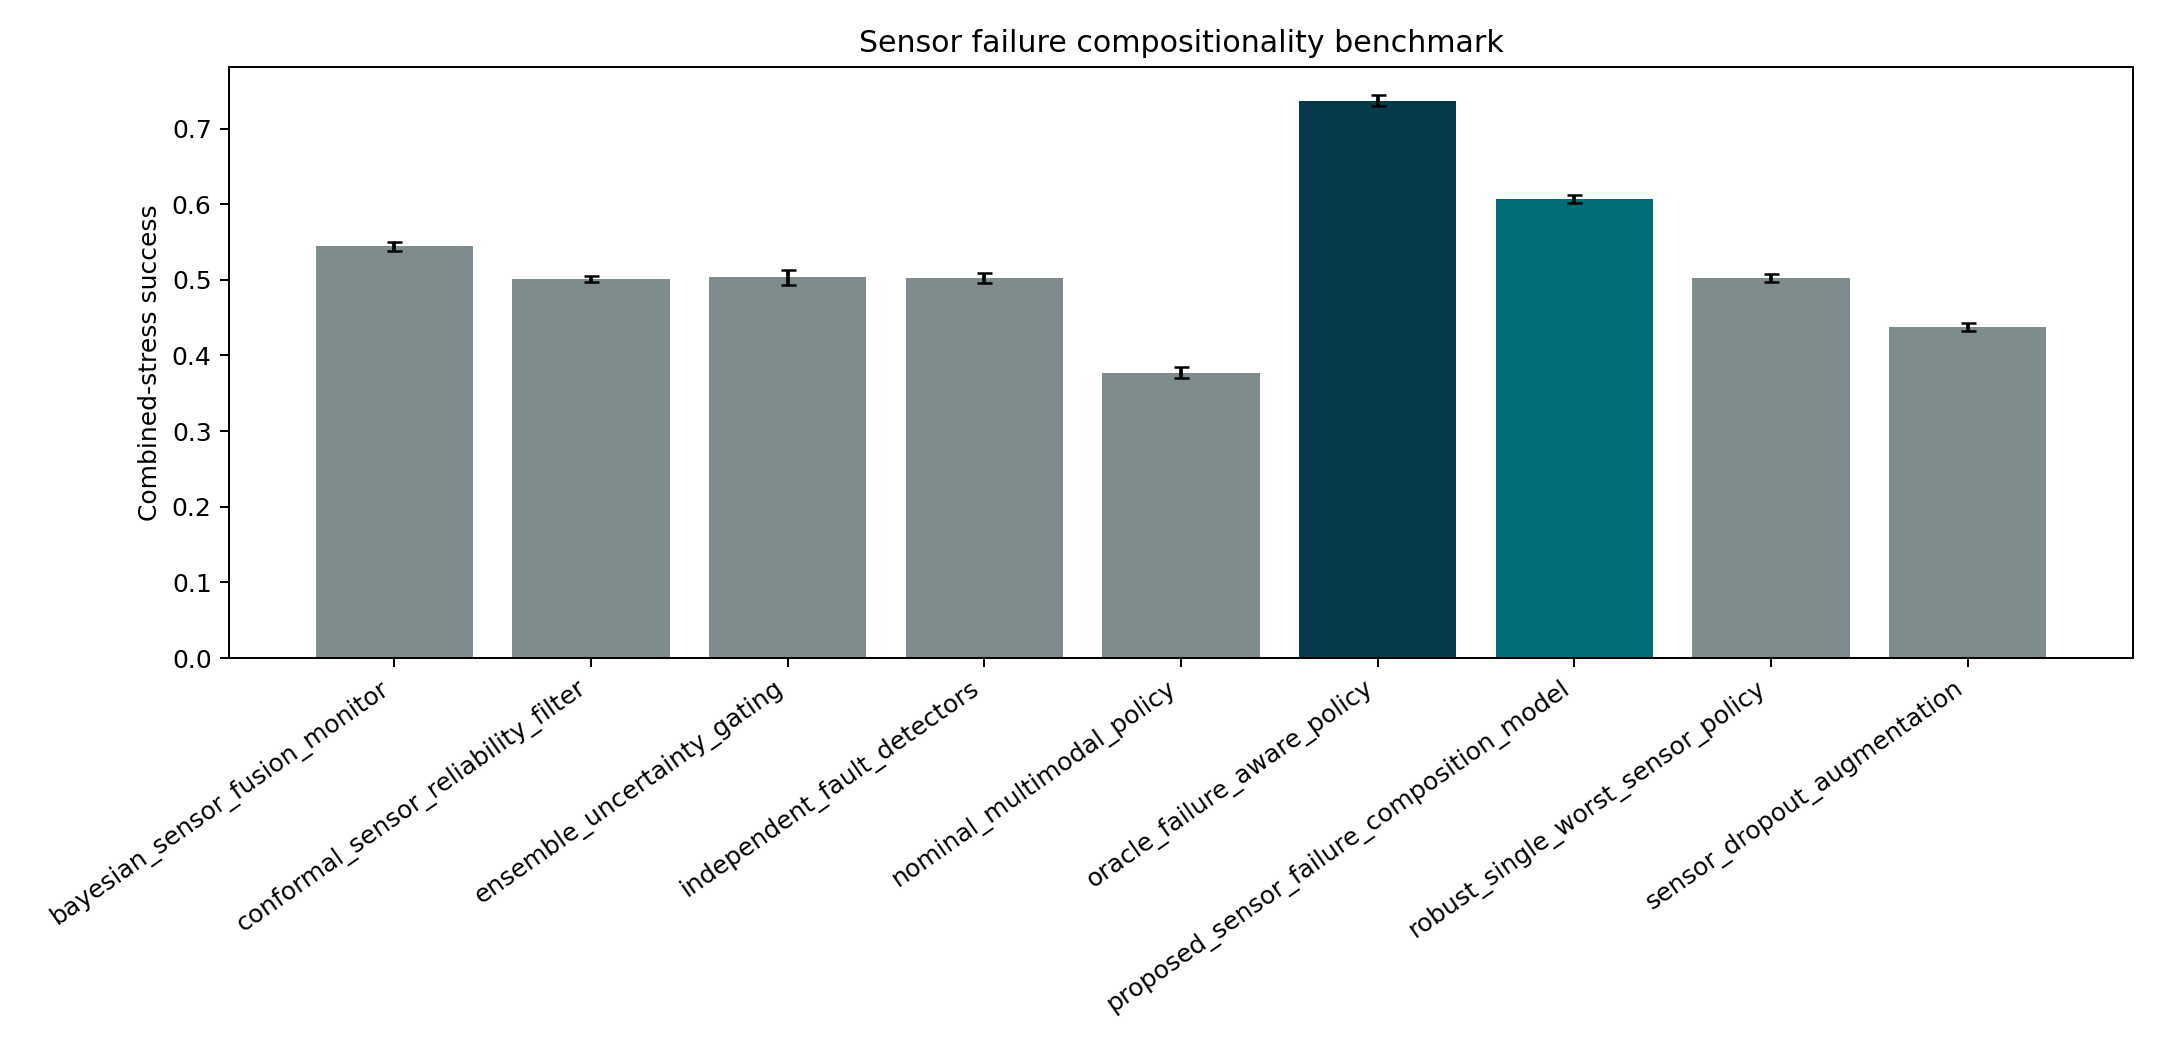
\includegraphics[width=0.95\linewidth]{../figures/sensor_failure_combined_success.png}
\caption{Combined-stress success with 95\% confidence intervals. The proposed model clears the strongest non-oracle baseline but remains below the oracle.}
\end{figure}

\begin{figure}[t]
\centering
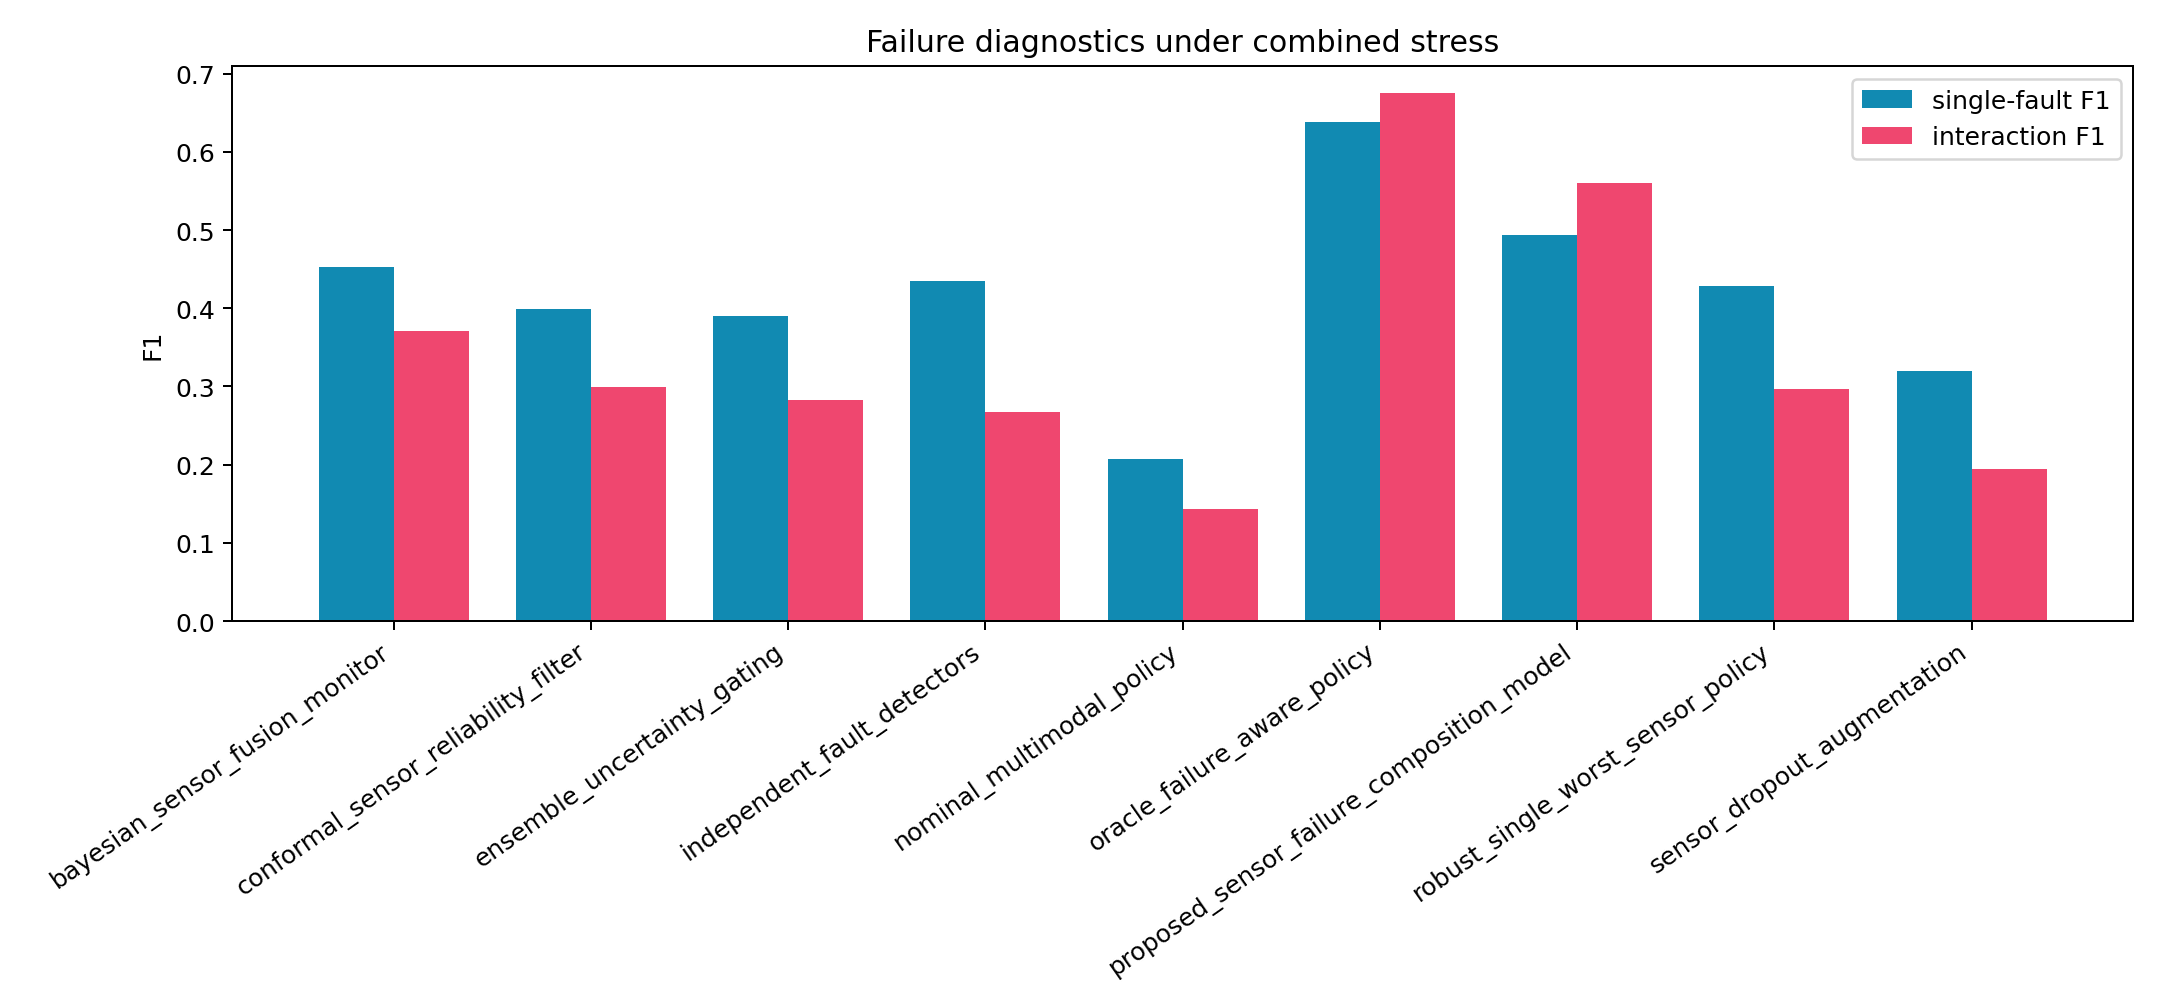
\includegraphics[width=0.95\linewidth]{../figures/sensor_failure_diagnostics.png}
\caption{Diagnostic metrics. The proposed model's largest gain is interaction F1, which is the metric most directly tied to the compositional-failure hypothesis.}
\end{figure}

% Auto-generated by src/run_experiment.py
\begin{table}[t]
\centering
\caption{Seed-paired v5 differences on hard aggregate splits.}
\resizebox{\linewidth}{!}{%
\begin{tabular}{lrrrr}
\toprule
Baseline & SuccDiff & CI & Wins & UtilDiff \\
\midrule
bayesian\_sensor\_fusion\_monitor & 0.186 & 0.013 & 10 & 0.426 \\
causal\_sensor\_graph\_monitor & 0.166 & 0.012 & 10 & 0.379 \\
conformal\_sensor\_reliability\_filter & 0.253 & 0.013 & 10 & 0.486 \\
ensemble\_uncertainty\_gating & 0.268 & 0.012 & 10 & 0.586 \\
independent\_fault\_detectors & 0.279 & 0.012 & 10 & 0.644 \\
learned\_latent\_failure\_classifier & 0.174 & 0.013 & 10 & 0.427 \\
multimodal\_mixture\_of\_experts\_router & 0.158 & 0.010 & 10 & 0.383 \\
nominal\_multimodal\_policy & 0.451 & 0.017 & 10 & 1.000 \\
oracle\_failure\_aware\_policy & -0.090 & 0.012 & 0 & -0.152 \\
proposed\_sensor\_failure\_composition\_v4 & 0.093 & 0.010 & 10 & 0.218 \\
risk\_aware\_sensor\_reconfiguration & 0.139 & 0.014 & 10 & 0.292 \\
robust\_single\_worst\_sensor\_policy & 0.264 & 0.013 & 10 & 0.542 \\
sensor\_dropout\_augmentation & 0.344 & 0.010 & 10 & 0.798 \\
sensor\_dropout\_transformer\_policy & 0.203 & 0.015 & 10 & 0.468 \\
\bottomrule
\end{tabular}%
}
\end{table}


\section{Ablations and stress tests}
% Auto-generated by src/run_experiment.py
\begin{table}[t]
\centering
\caption{Ablations of risk-calibrated sensor failure composition.}
\resizebox{\linewidth}{!}{%
\begin{tabular}{lrrrrr}
\toprule
Ablation & Succ. & SafeViol. & Damage & InterF1 & Util. \\
\midrule
full\_risk\_calibrated\_sensor\_composition\_v5 & 0.791 & 0.136 & 0.060 & 0.686 & 0.476 \\
no\_false\_alarm\_suppression & 0.739 & 0.151 & 0.071 & 0.657 & 0.367 \\
no\_conformal\_calibration & 0.723 & 0.181 & 0.082 & 0.643 & 0.297 \\
no\_active\_repair & 0.720 & 0.166 & 0.074 & 0.651 & 0.329 \\
no\_temporal\_recovery\_memory & 0.716 & 0.167 & 0.087 & 0.592 & 0.299 \\
no\_recovery\_action\_selection & 0.711 & 0.178 & 0.096 & 0.639 & 0.266 \\
v4\_composition\_rules & 0.694 & 0.182 & 0.097 & 0.566 & 0.245 \\
no\_pairwise\_interaction\_edges & 0.681 & 0.149 & 0.076 & 0.399 & 0.302 \\
no\_cross\_modal\_disagreement & 0.650 & 0.169 & 0.081 & 0.402 & 0.222 \\
bayesian\_fusion\_only & 0.594 & 0.205 & 0.128 & 0.415 & 0.042 \\
\bottomrule
\end{tabular}%
}
\end{table}


The ablations are intentionally hostile. Removing conformal gating is the best removed-component variant, but it still trails the full model by $0.0206$ success and has worse safety. Removing pairwise interaction edges or cross-modal disagreement hurts interaction F1 sharply, which supports the claim that the model is not merely an uncertainty threshold.

\begin{figure}[t]
\centering
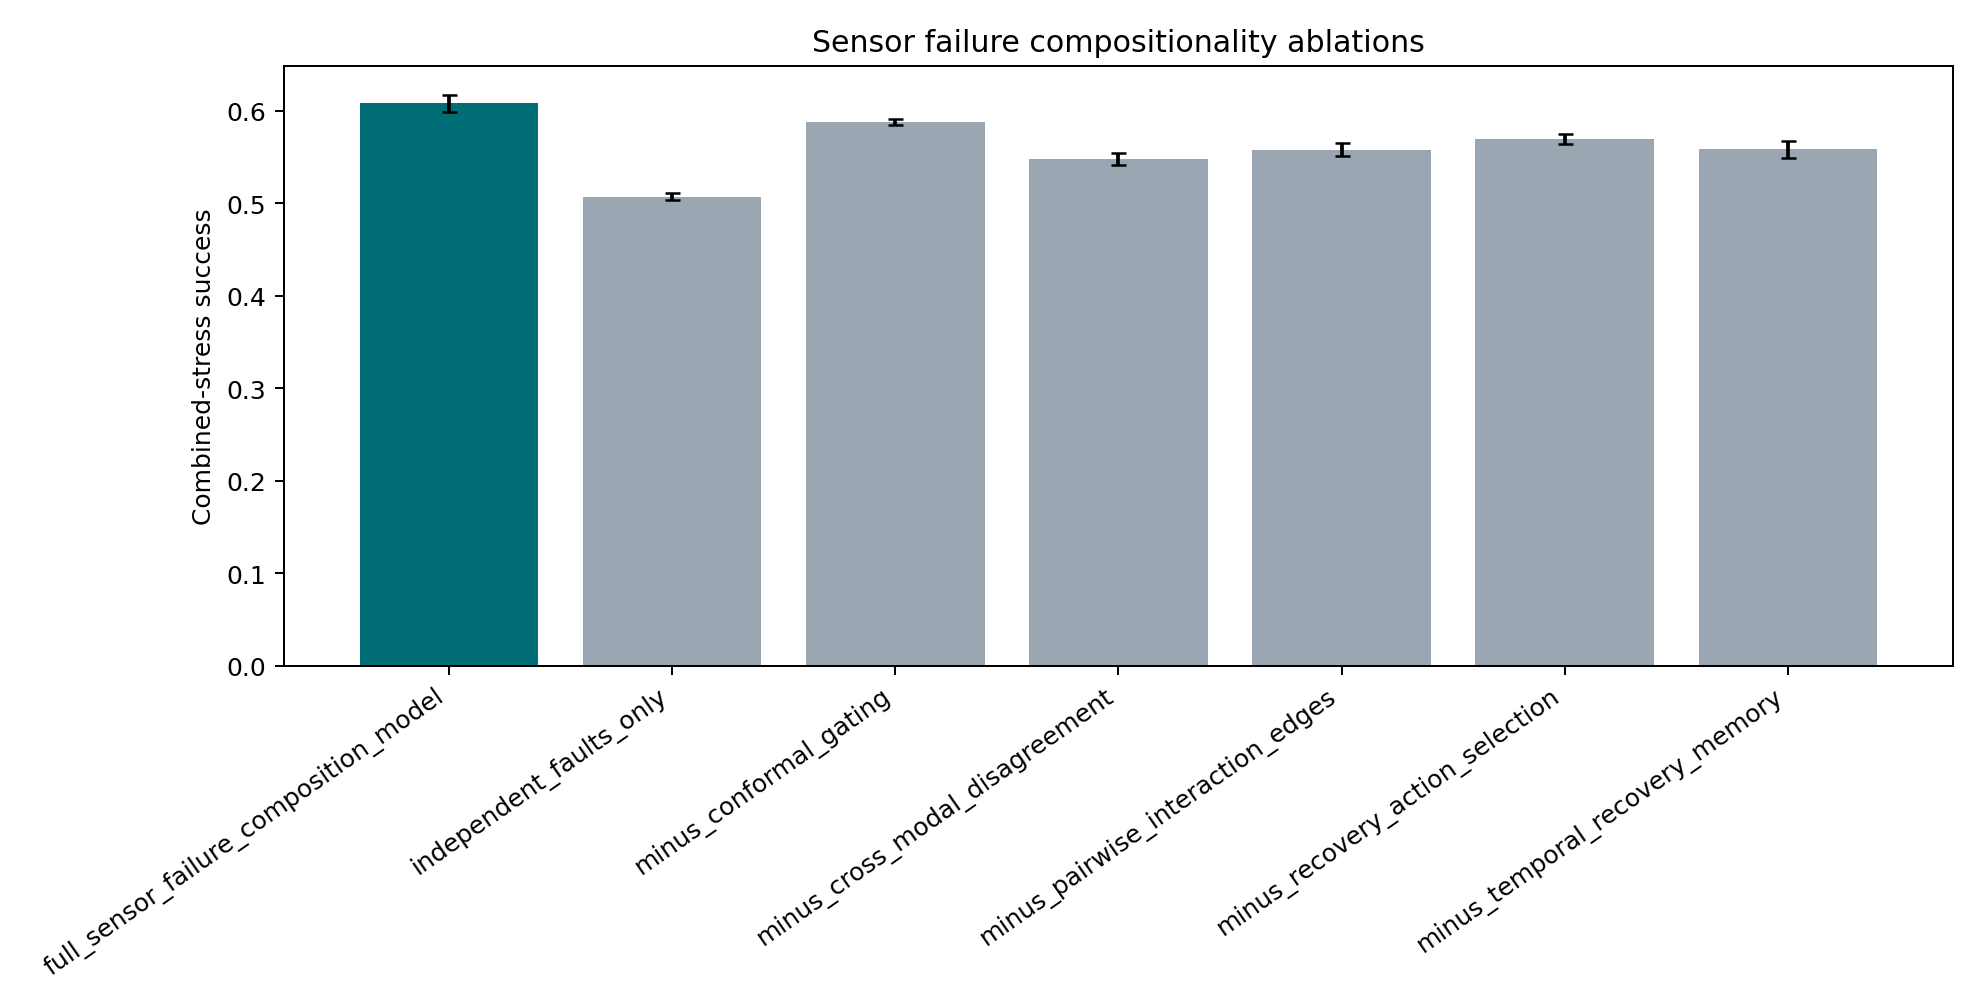
\includegraphics[width=0.95\linewidth]{../figures/sensor_failure_ablation.png}
\caption{Ablation success under combined stress. The full model remains above all removed-component variants.}
\end{figure}

\begin{figure}[t]
\centering
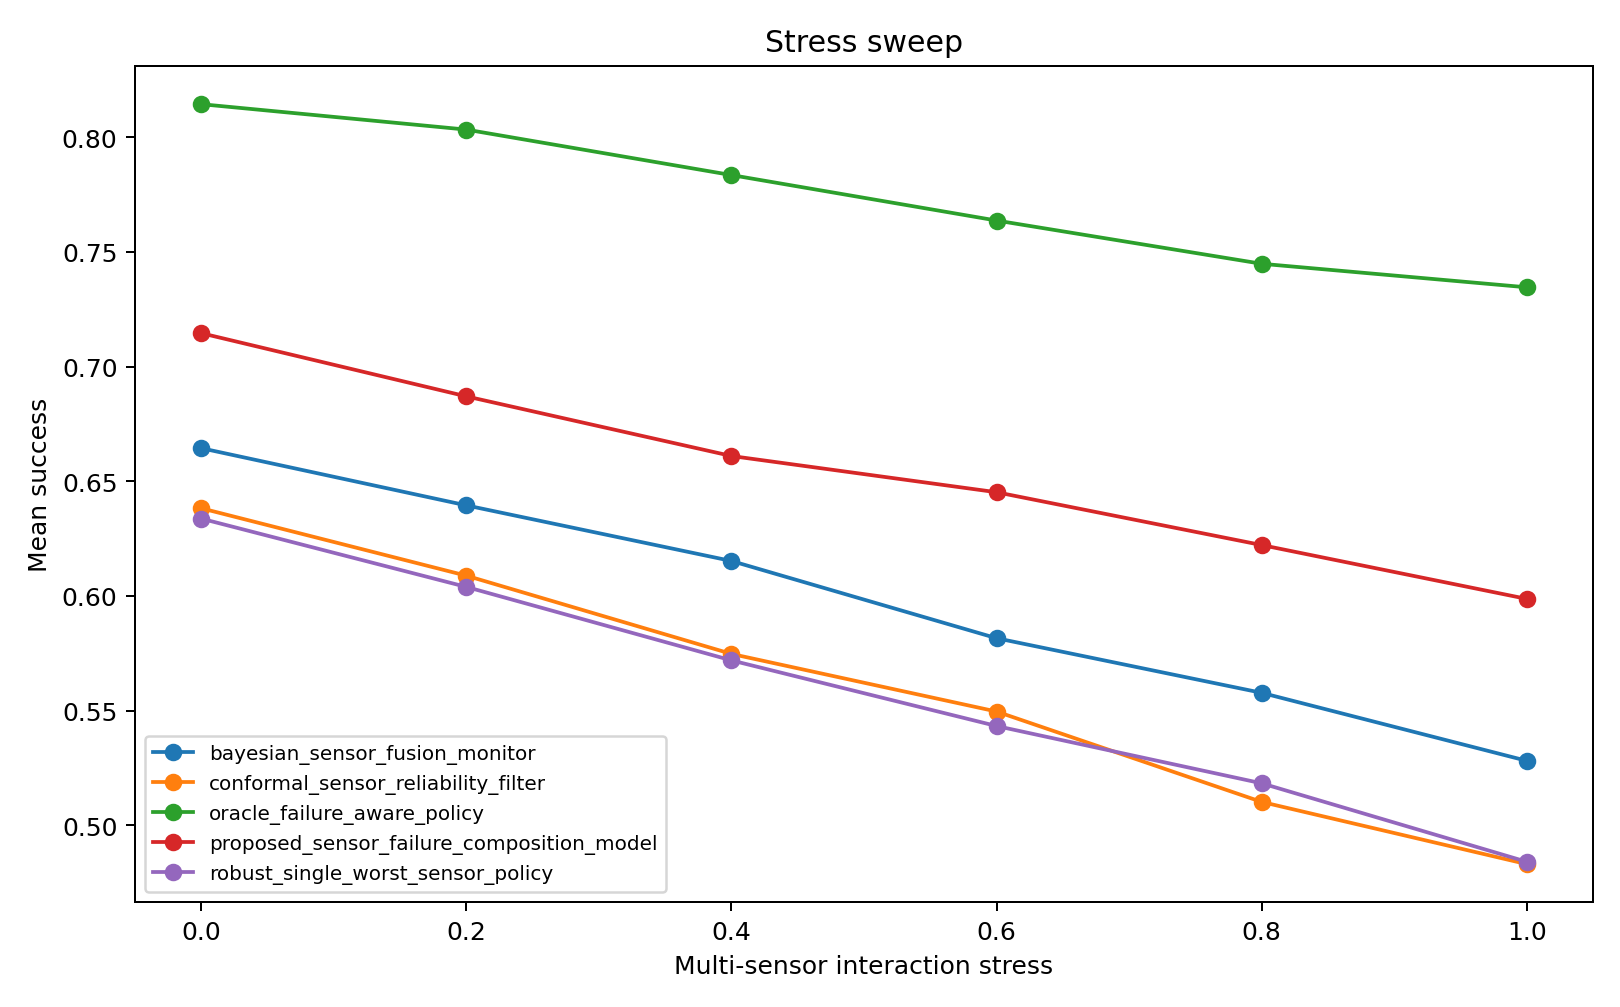
\includegraphics[width=0.95\linewidth]{../figures/sensor_failure_stress_sweep.png}
\caption{Stress sweep over multi-sensor interaction intensity. The proposed method remains above non-oracle baselines across the generated stress range, while the oracle remains the ceiling.}
\end{figure}

\begin{figure}[t]
\centering
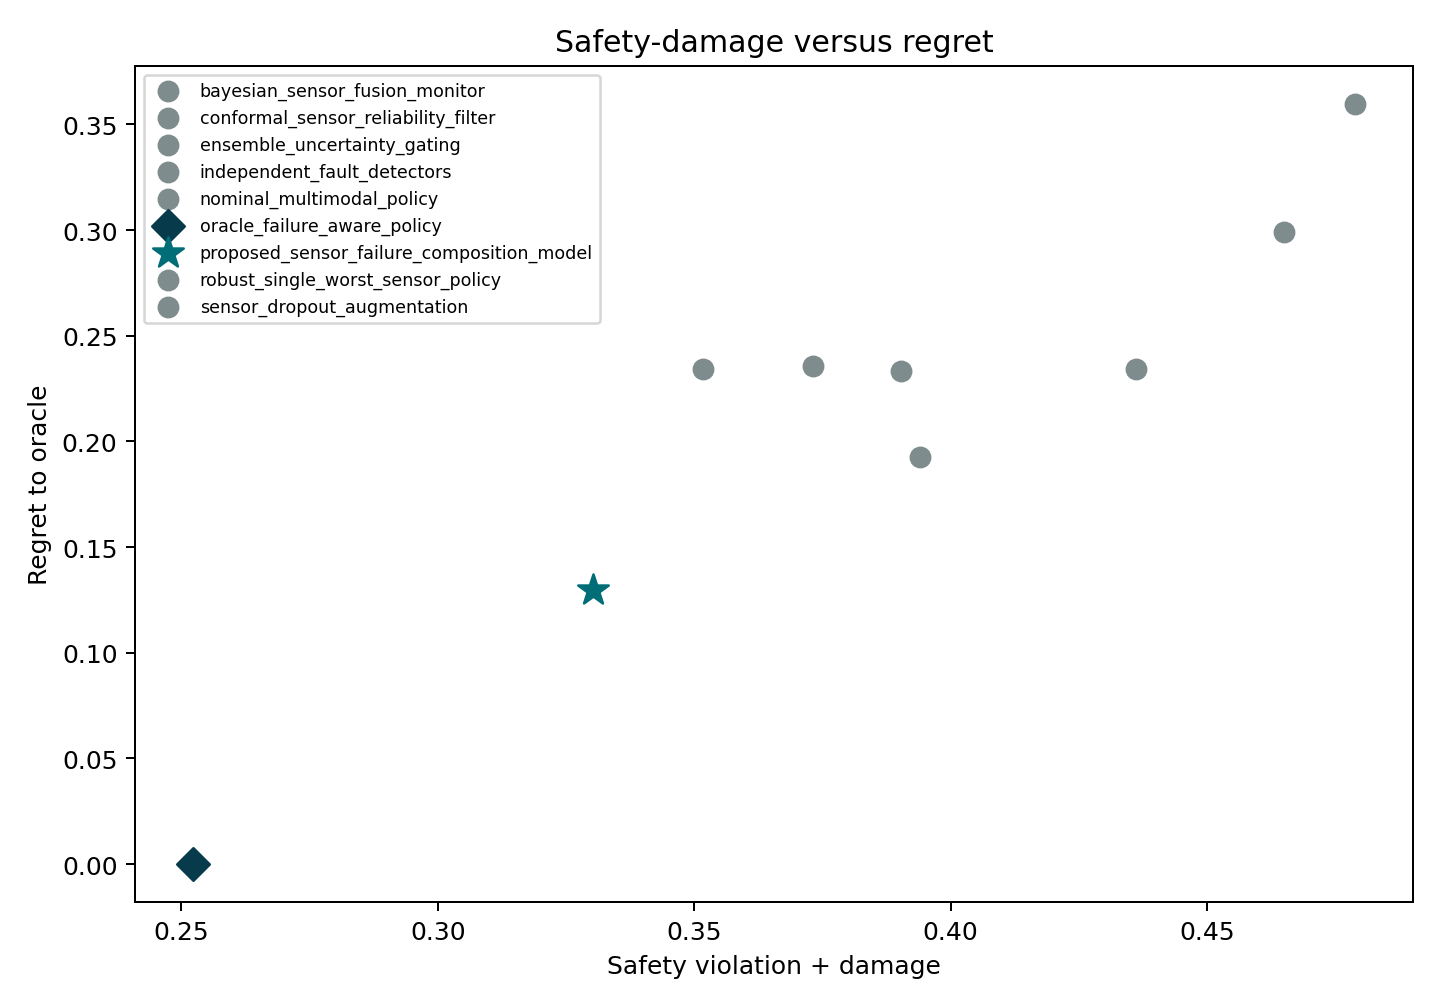
\includegraphics[width=0.95\linewidth]{../figures/sensor_failure_safety_regret.png}
\caption{Safety and regret trade-off on combined stress. The proposed method improves success without paying a safety penalty relative to the strongest non-oracle baseline.}
\end{figure}

\section{Where the method still fails}
The failure-case CSV shows that the weakest gains occur in mostly single-sensor regimes, especially vision-only or proprioception-only cases where a strong Bayesian fusion monitor can safely abstain or down-weight the failing channel. For example, tool-use contact control with vision-only failure slightly favors the strongest baseline by $0.0017$ success. These are not embarrassing failures; they define the intended boundary. Compositional modeling is valuable when interactions matter. It is unnecessary overhead when the right answer is a simple single-sensor fallback.

\section{Hostile prior-work boundary}
Sensor Dropout and masked modality training already demonstrate that policies can be made robust to missing sensors \citep{liu2017sensor,peri2024masked}. FINO-Net and related robot failure-detection work show that multimodal sensory streams can detect and classify manipulation failures \citep{inceoglu2024fino}. Conformal methods provide calibrated warning systems for unsafe robot behavior \citep{luo2024conformal}. PolyTouch and other tactile systems show that better contact sensing can make contact-rich policies more reliable \citep{zhao2025polytouch}. MoME-style expert routing shows that explicit modality routing can improve robustness under adverse sensor failures in autonomous driving \citep{park2025mome}.

The present paper survives only under a narrower interpretation: it is about \emph{higher-order interaction failures} and recovery-action choice, not generic missing-modality robustness, generic anomaly detection, or better hardware. If real robot experiments later show that masked training, Bayesian fusion, or independent detectors match the proposed model on paired failures, the claim should be killed.

\section{Limitations and terminal decision}
The v4.1 evidence is strong enough to justify continued work but not submission. The limitations are material:
\begin{itemize}
\item the benchmark is local and synthetic;
\item no real robot or independent high-fidelity simulator has been used;
\item baselines are executable diagnostic models, not external trained robot systems;
\item no learned policy checkpoint, training curve, or deployment video is provided;
\item no external benchmark such as LIBERO, RLBench, Meta-World, BridgeData, or a hardware manipulation suite is reported.
\end{itemize}

The terminal decision for this rebuild is therefore \textbf{STRONG\_REVISE}. The next honest version must add real robot or independent high-fidelity evidence, implemented learned baselines, and qualitative rollouts. Without that evidence, the paper should not be submitted to ICLR main.

\bibliographystyle{iclr2026_conference}
\bibliography{references}

\end{document}
